\begin{figure}
\centering	
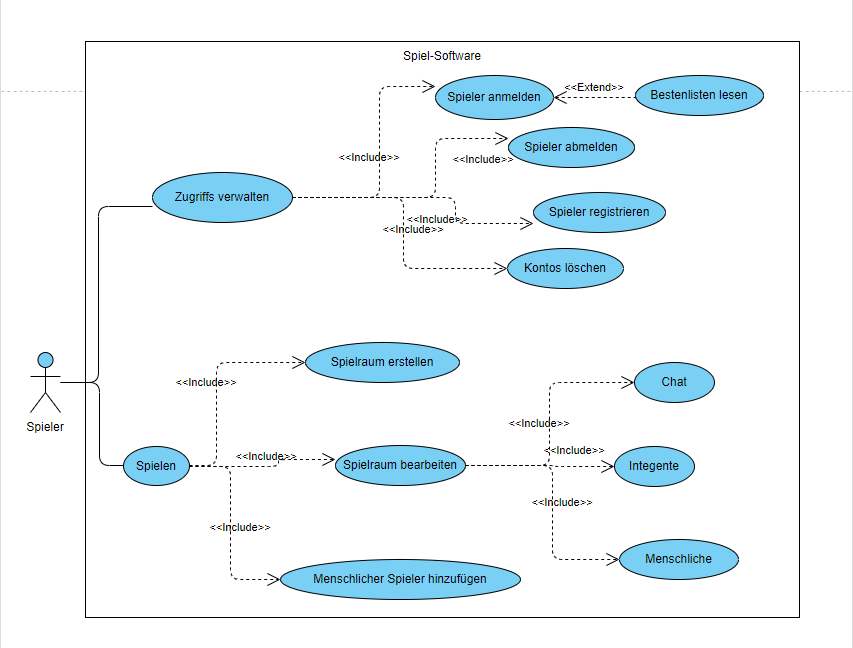
\includegraphics[width=0.9\textwidth]{img/group6.png}
\label{fig:sys}
\caption{Use Case Diagramm}
\end{figure}

\section{Systemgrenze (Use Case Diagramm)}

Die Systemgrenze wird in der Abbildung~\ref{fig:sys} dargestellt. 


\section{Beschreibungen der Anwendungsfälle}


\newcounter{uc}\setcounter{uc}{10}

\begin{description}[leftmargin=5em, style=sameline]

	\begin{lhp}{uc}{UC}{uc:zugriff}
		\item [Name:] Zugriff verwalten.
		\item [Ziel:] Zugriffsverwaltung.
		\item [Akteure:] Das System.
		\item [Vorbedingungen:] Falls vorhanden, Benutzername und Passwort. Falls nicht vorhanden, keine.
		\item [Eingabedaten:] Falls vorhanden, Benutzername \ref{daten:benutzername} und Passwort \ref{daten:passwort}. Falls nicht vorhanden, keine.
		\item [Beschreibung:] \hfill\\ Falls schon registriert:\hfill\\
		1. Der Spieler gibt der Benutzername und das Passwort.\\
		2. System prüft die Richtigkeit der Daten.\\
		\hfill\\ Falls nicht registriert:\hfill\\
		siehe \ref{uc:registrieren}
		\item [Ausnahmen:] \hfill
		\begin{itemize} 
		\item[] \textit{Benutzername und Passwort passen nicht zusammen:} Das System gibt dem Spieler einen Hinweis.				\item[] \textit{Noch nicht registriert:} siehe \ref{uc:registrieren}.
		
	\end{itemize}
	
		\item [Ergebnisse und Outputdaten:] Das Spieler hat sich erfolgreich angemeldet.
		\item [Systemfunktionen] \ref{funk:zugriff}.
	\end{lhp}

	\begin{lhp}{uc}{UC}{uc:registrieren}
	    \item [Name:] Spieler registieren.
	    \item [Ziel:] Spieler registiert sich.
	    \item [Akteure:] Spieler.
	    \item [Vorbedingungen] Keine.
        \item [Eingabedaten:] Name\ref{daten:benutzername}, Passwort\ref{daten:passwort}, Email\ref{daten:email}. 
	\item [Beschreibung:] \hfill\\ \hfill\\
	1. Spieler sendet das Formular ab.\\
	2. Das System prüft ob der Benutzername schon vorhanden ist\\	
	3. Spieler erfolgreich registiert.\\			
	\item [Ausnahmen:]\hfill 
	\begin{itemize} 
		\item[] \textit{Benutzername schon vorhanden:} Das System zeigt eine Fehlermeldung an und Spieler sendet das Formular mit anderem Benutzername ab.					
		
	\end{itemize}
	\item [Ergebnisse und Outputdaten:] Spieler erfolgreich registiert.	
	\item [Systemfunktionen:] \ref{funk:zugriff}.
    \end{lhp}
	
	\begin{lhp}{uc}{UC}{uc:anmeld}
		\item [Name:] Spieler anmelden.
		\item [Ziel:] Spieler meldet sich im System an.
		\item [Akteure:] Spieler.
		\item [Vorbedingungen] Spieler ist erfolgreich angemeldet.
		\item [Eingabedaten:] Zugriffsdaten~\ref{daten:benutzername}~\ref{daten:passwort}.
		\item [Beschreibung:] \hfill\\ \hfill\\
			1. Spieler sendet das Formular ab.\\
			2. Das System prüft die Gültigkeit von Zugangsdaten.\\				
		\item [Ausnahmen:]\hfill 
	    	\begin{itemize} 
			    \item[] \textit{Passwort oder Benutzername ist falsch:} Das System zeigt eine Fehlermeldung an.					
			
		    \end{itemize}
		\item [Ergebnisse und Outputdaten:] Spieler erfolgreich angemeldet.	
		\item [Systemfunktionen:] \ref{funk:zugriff}.
	\end{lhp}
	
	\begin{lhp}{uc}{UC}{uc:namechange}
		\item [Name:] Benutzername ändern.
		\item [Ziel:] Spieler ändert seinen Benutzername.
		\item [Akteure:] Spieler.
		\item [Vorbedingungen] Spieler ist erfolgreich angemeldet.
		\item [Eingabedaten:] Zugriffsdaten~\ref{daten:benutzername}~\ref{daten:passwort}.
		\item [Beschreibung:] \hfill\\ \hfill\\
			1. Spieler sendet das Formular ab.\\
			2. Das System prüft die Gültigkeit von Zugangsdaten.\\				
		\item [Ausnahmen:]\hfill 
	    	\begin{itemize} 
			    \item[] \textit{Passwort ist falsch:} Das System zeigt eine Fehlermeldung an.					
			
		    \end{itemize}
		\item [Ergebnisse und Outputdaten:] Benutzername erfolgreich geändert.	
		\item [Systemfunktionen:] \ref{funk:accountverw}.
	\end{lhp}	
	
	\begin{lhp}{uc}{UC}{uc:pwchange}
		\item [Name:] Passwort ändern.
		\item [Ziel:] Spieler ändert sein Passwort.
		\item [Akteure:] Spieler.
		\item [Vorbedingungen] Spieler ist erfolgreich angemeldet.
		\item [Eingabedaten:] Passwort~\ref{daten:passwort}.
		\item [Beschreibung:] \hfill\\ \hfill\\
			1. Spieler sendet das Formular ab.\\
			2. Das System prüft die Gültigkeit des Passworts.\\				
		\item [Ausnahmen:]\hfill 
	    	\begin{itemize} 
			    \item[] \textit{Passwort ist falsch:} Das System zeigt eine Fehlermeldung an.					
			
		    \end{itemize}
		\item [Ergebnisse und Outputdaten:] Passwort erfolgreich geändert.	
		\item [Systemfunktionen:] \ref{funk:accountverw}.
	\end{lhp}	
	
	\begin{lhp}{uc}{UC}{uc:loeschen}
		\item [Name:] Spieler löschen.
		\item [Ziel:] Spieler entfernt seine Daten aus dem System.
		\item [Akteure:] Spieler.
		\item [Vorbedingungen] Spieler erfolgreich angemeldet.
		\item [Eingabedaten:] Passwort~\ref{daten:passwort}.
		\item [Beschreibung:] \hfill\\ \hfill\\
				1. Spieler sendet das Formular ab.\\
				2. Das System prüft die Richtigkeit des Passworts und fragt Spieler noch ein mal, ob er sich wirklich aus dem System entfernen möchte.\\
				3. Spieler bestätigt seine Intention.\\
				4. Das System entfernt alle Daten des Spielers aus der Datenbank und bewegt Spieler in den Vorraum.\\
		\item [Ausnahmen:] \hfill
			\begin{itemize} 
				\item[] \textit{Keine Löschung erwünscht:} Schritt 4 wird nicht durchgeführt.
				
			\end{itemize}
		\item [Ergebnisse und Outputdaten:] Spielerkonto wurde gelöscht.	
		\item [Systemfunktionen:] \ref{funk:zugriff}.
	\end{lhp}
   
	\begin{lhp}{uc}{UC}{uc:bestenlistesehen}
    	\item [Name:] Bestenliste lesen.
    	\item [Ziel:] Spieler liest die Bestenliste.
    	\item [Akteure:] Spieler.
    	\item [Vorbedingungen] Spieler erfolgreich angemeldet.
    	\item [Eingabedaten:] keine.
    	\item [Beschreibung:] Spieler liest die Bestenliste \ref{daten:bestenliste}.
    	\item [Ausnahmen:] keine.
    	\item [Ergebnisse und Outputdaten:] Die Bestenliste wird angezeigt.	
    	\item [Systemfunktionen:] \ref{funk:bestenliste}.
    \end{lhp}

	\begin{lhp}{uc}{UC}{uc:spielen}
     	\item [Name:] Spielraum betreten.
    	\item [Ziel:] Spieler betritt Spielraum.
	    \item [Akteure:] Spieler.
    	\item [Vorbedingungen] Spieler erfolgreich angemeldet.
    	\item [Eingabedaten:] keine.
    	\item [Beschreibung:] \hfill\\ \hfill\\
    	1. Spieler wählt einen Spielraum aus und will diesem beitreten.\\
    	2. System prüft ob Spieler dem Raum beitreten kann.\\
    	3. Spieler tritt dem Raum bei oder bekommt eine Fehlermeldung.\\
    	\item [Ausnahmen:] \hfill
    	\begin{itemize} 
				\item[] \textit{Raum ist voll:} Spieler erhält eine Fehlermeldung.
				
			\end{itemize}
    	\item [Ergebnisse und Outputdaten:] Spieler in einen Spielraum.
     	\item [Systemfunktionen:] \ref{funk:spielraum}.
    \end{lhp} 

    \begin{lhp}{uc}{UC}{uc:chat}
    	\item [Name:] Chatten.
    	\item [Ziel:] Spieler chat mit einander.
    	\item [Akteure:] Spieler.
    	\item [Vorbedingungen] Spieler erfolgreich angemeldet und steht in einem Spielraum. 
    	\item [Eingabedaten:] Chatnachricht.
    	\item [Beschreibung:] \hfill\\ \hfill\\
    	1. Spieler sendet eine Nachricht.\\
    	2. System sendet Nachricht an andere Spieler.\\
    	\item [Ausnahmen:] \hfill
    	\begin{itemize} 
				\item[] \textit{Nachricht ist leer:} Schritt 2 wird übersprungen.
				
			\end{itemize}
    	\item [Ergebnisse und Outputdaten:] Chatnachricht.
    	\item [Systemfunktionen:] \ref{funk:chat}.
    \end{lhp}


    \begin{lhp}{uc}{UC}{uc:intelligentbots}
    	\item [Name:] Intelligente Bots hinzufügen.
    	\item [Ziel:] Spieler fügt ein Bot Spieler zum Spielraum.
    	\item [Akteure:] Spieler.
    	\item [Vorbedingungen] Spieler ist in einem Spielraum. 
      	\item [Eingabedaten:] keine.
    	\item [Beschreibung:] \hfill\\ \hfill\\
    	1. Spieler will einen Bot Spieler zum Spiel hinzufügen.\\
    	2. System fragt nach der Stärke des Bots.\\
    	3. Spieler gibt Präferenzen an.\\
    	4. System fügt Bot hinzu.\\
    	\item [Ausnahmen:] \hfill
    	\begin{itemize} 
				\item[] \textit{Raum ist voll:} Spieler erhält eine Fehlermeldung.
				
			\end{itemize} 
    	\item [Ergebnisse und Outputdaten:] Bot erfolgreich hinzugefügt.
    	\item [Systemfunktionen:] \ref{funk:bots}.
    \end{lhp}
    
        \begin{lhp}{uc}{UC}{uc:spielstart}
    	\item [Name:] Spielstart
    	\item [Ziel:] Alle Spieler bekommen ihre Handkarten zugeteilt und das Spiel beginnt.
    	\item [Akteure:] Spieler.
    	\item [Vorbedingungen] Spieler ist in einem Spiel. 
      	\item [Eingabedaten:] Gewünschte Karte(n).
    	\item [Beschreibung:] \hfill\\ \hfill\\
    	1. Spieler startet das Spiel aus der Lobby.\\
    	2. System gibt jedem Spieler seine 8 Handkarten und bereitet den Spielstapel vor.\\
    	3. Ein zufälliger Spieler beginnt mit seinem ersten Zug, danach geht es im Uhrzeigersinn weiter.\\
    	\item [Ausnahmen:] \hfill
    	\begin{itemize} 
				\item[] \textit{Nicht genug Spieler im Spielraum:} Spiel kann nicht gestartet werden.
				
			\end{itemize} 
    	\item [Ergebnisse und Outputdaten:] Handkarten und Spielstapel sind regelkonform aufgeteilt.
    	\item [Systemfunktionen:] \ref{funk:spielverw}.
    \end{lhp}
    
    \begin{lhp}{uc}{UC}{uc:kartelegen}
    	\item [Name:] Karte(n) legen
    	\item [Ziel:] Spieler legt Karte(n) von seiner Hand auf den Ablagestapel.
    	\item [Akteure:] Spieler.
    	\item [Vorbedingungen] Spieler ist in einem Spiel. 
      	\item [Eingabedaten:] Gewünschte Karte(n).
    	\item [Beschreibung:] \hfill\\ \hfill\\
    	1. Spieler will Karte(n) aus seiner Hand ablegen.\\
    	2. System prüft ob keine Regel verletzt wird.\\
    	3. Spieler legt Karte(n) ab.\\
    	\item [Ausnahmen:] \hfill
    	\begin{itemize} 
				\item[] \textit{Aktion widerspricht den Regeln:} Spieler erhält eine Fehlermeldung.
				
			\end{itemize} 
    	\item [Ergebnisse und Outputdaten:] Karte(n) werden abgelegt und ihr Effekt ausgeführt.
    	\item [Systemfunktionen:] \ref{funk:spielverw}.
    \end{lhp}

    \begin{lhp}{uc}{UC}{uc:zugbeenden}
    	\item [Name:] Zug beenden
    	\item [Ziel:] Spieler beendet seinen Zug.
    	\item [Akteure:] Spieler.
    	\item [Vorbedingungen] Spieler ist in einem Spiel. Spieler ist am Zug.
      	\item [Eingabedaten:] keine
    	\item [Beschreibung:] \hfill\\ \hfill\\
    	1. Spieler will seinen Zug beenden.\\
    	2. System prüft ob keine Regel verletzt wird.\\
    	3. Spieler beendet seinen Zug und zieht eine Karte.\\
    	\item [Ausnahmen:] \hfill
    	\begin{itemize} 
				\item[] \textit{Aktion widerspricht den Regeln:} Spieler erhält eine Fehlermeldung.
				
			\end{itemize} 
    	\item [Ergebnisse und Outputdaten:] Spieler beendet seinen Zug und zieht eine Karte.
    	\item [Systemfunktionen:] \ref{funk:spielverw}.
    \end{lhp}

	\begin{lhp}{uc}{UC}{uc:entschärfen}
    	\item [Name:] Entschärfen
    	\item [Ziel:] Spieler entschärft ein Exploding Kitten.
    	\item [Akteure:] Spieler.
    	\item [Vorbedingungen] Spieler ist in einem Spiel. Spieler hat Exploding Kitten auf der Hand.
      	\item [Eingabedaten:] keine
    	\item [Beschreibung:] \hfill\\ \hfill\\
    	1. Spieler will eine Entschärfung spielen.\\
    	2. System prüft ob keine Regel verletzt wird.\\
    	3. Spieler entschärft das Exploding Kitten und legt es zurück in den Spielstapel.\\
    	\item [Ausnahmen:] \hfill
    	\begin{itemize} 
				\item[] \textit{Aktion widerspricht den Regeln:} Spieler erhält eine Fehlermeldung.
				\item[] \textit{Spieler besitzt keine Entschärfung:} Spieler erhält eine Fehlermeldung.
			\end{itemize} 
    	\item [Ergebnisse und Outputdaten:] Spieler legt Entschärfung auf den Ablagestapel und Exploding Kitten in den Spielstapel.
    	\item [Systemfunktionen:] \ref{funk:spielverw}.
    \end{lhp}
    
    \begin{lhp}{uc}{UC}{uc:ausscheiden}
    	\item [Name:] Ausscheiden
    	\item [Ziel:] Spieler scheidet aus dem Spiel aus.
    	\item [Akteure:] Spieler.
    	\item [Vorbedingungen] Spieler ist in einem Spiel. Spieler kann nicht Entschärfen und hat ein Exploding Kitten auf der Hand.
      	\item [Eingabedaten:] keine
    	\item [Beschreibung:] \hfill\\ \hfill\\
    	1. Spieler hat keine gültigen Aktionen mehr.\\
    	2. System legt alle Karten von der Hand des Spielers auf den Ablagestapel.\\
    	\item [Ausnahmen:] keine
    	\item [Ergebnisse und Outputdaten:] Spieler scheidet aus dem Spiel aus und legt alle seine Karten auf den Ablagestapel.
    	\item [Systemfunktionen:] \ref{funk:spielverw}.
    \end{lhp}

 	\begin{lhp}{uc}{UC}{uc:spielende}
    	\item [Name:] Spielende
    	\item [Ziel:] Spiel wird beendet.
    	\item [Akteure:] Spieler.
    	\item [Vorbedingungen] Spieler ist in einem Spiel. Vorletzter Spieler ist ausgeschieden.
      	\item [Eingabedaten:] keine
    	\item [Beschreibung:] \hfill\\ \hfill\\
    	1. Nur noch ein Spieler ist am leben.\\
    	2. System weist diesem Spieler seine Punkte für die Bestenliste zu und schickt die Spieler zurück in die Lobby.\\
    	\item [Ausnahmen:] keine
    	\item [Ergebnisse und Outputdaten:] Spieler gewinnt das Spiel und kehrt in die Lobby zurück.
    	Bestenliste wird upgedatet.
    	\item [Systemfunktionen:] \ref{funk:spielverw}, \ref{funk:bestenliste}.
    \end{lhp}
    
\end{description}